%% Based on a TeXnicCenter-Template by Gyorgy SZEIDL.
%%%%%%%%%%%%%%%%%%%%%%%%%%%%%%%%%%%%%%%%%%%%%%%%%%%%%%%%%%%%%

%------------------------------------------------------------
%
\documentclass{article}%
%Options -- Point size:  10pt (default), 11pt, 12pt
%        -- Paper size:  letterpaper (default), a4paper, a5paper, b5paper
%                        legalpaper, executivepaper
%        -- Orientation  (portrait is the default)
%                        landscape
%        -- Print size:  oneside (default), twoside
%        -- Quality      final(default), draft
%        -- Title page   notitlepage, titlepage(default)
%        -- Columns      onecolumn(default), twocolumn
%        -- Equation numbering (equation numbers on the right is the default)
%                        leqno
%        -- Displayed equations (centered is the default)
%                        fleqn (equations start at the same distance from the right side)
%        -- Open bibliography style (closed is the default)
%                        openbib
% For instance the command
%           \documentclass[a4paper,12pt,leqno]{article}
% ensures that the paper size is a4, the fonts are typeset at the size 12p
% and the equation numbers are on the left side
%
\usepackage{amsmath}%
\usepackage{amsfonts}%
\usepackage{amssymb}%
\usepackage{graphicx}
%-------------------------------------------
\newtheorem{theorem}{Theorem}
\newtheorem{acknowledgement}[theorem]{Acknowledgement}
\newtheorem{algorithm}[theorem]{Algorithm}
\newtheorem{axiom}[theorem]{Axiom}
\newtheorem{case}[theorem]{Case}
\newtheorem{claim}[theorem]{Claim}
\newtheorem{conclusion}[theorem]{Conclusion}
\newtheorem{condition}[theorem]{Condition}
\newtheorem{conjecture}[theorem]{Conjecture}
\newtheorem{corollary}[theorem]{Corollary}
\newtheorem{criterion}[theorem]{Criterion}
\newtheorem{definition}[theorem]{Definition}
\newtheorem{example}[theorem]{Example}
\newtheorem{exercise}[theorem]{Exercise}
\newtheorem{lemma}[theorem]{Lemma}
\newtheorem{notation}[theorem]{Notation}
\newtheorem{problem}[theorem]{Problem}
\newtheorem{proposition}[theorem]{Proposition}
\newtheorem{remark}[theorem]{Remark}
\newtheorem{solution}[theorem]{Solution}
\newtheorem{summary}[theorem]{Summary}
\newenvironment{proof}[1][Proof]{\textbf{#1.} }{\ \rule{0.5em}{0.5em}}

\begin{document}

\begin{flushleft}
\textbf{Course:} CSC 520, Introduction to Artificial Intelligence\\
\textbf{Homework 3}\\
\textbf{Student: Xusheng Xiao} \\
\textbf{Unity ID: xxiao2} \\
\textbf{Email: xxiao2@ncsu.edu}
\end{flushleft}

\noindent{\hrulefill}

\bigskip

\begin{enumerate}
	\item (80 pts.) This question concerns route-finding, with comparison of several search algorithms. This time, we're in the U.S. Here's jpg of the map below. The solution consists of the series of cities the agent must pass through, each city connected to one or more others by roads of the indicated length. There are no other roads. 
	
	\begin{figure}[h]
	\begin{center}
  	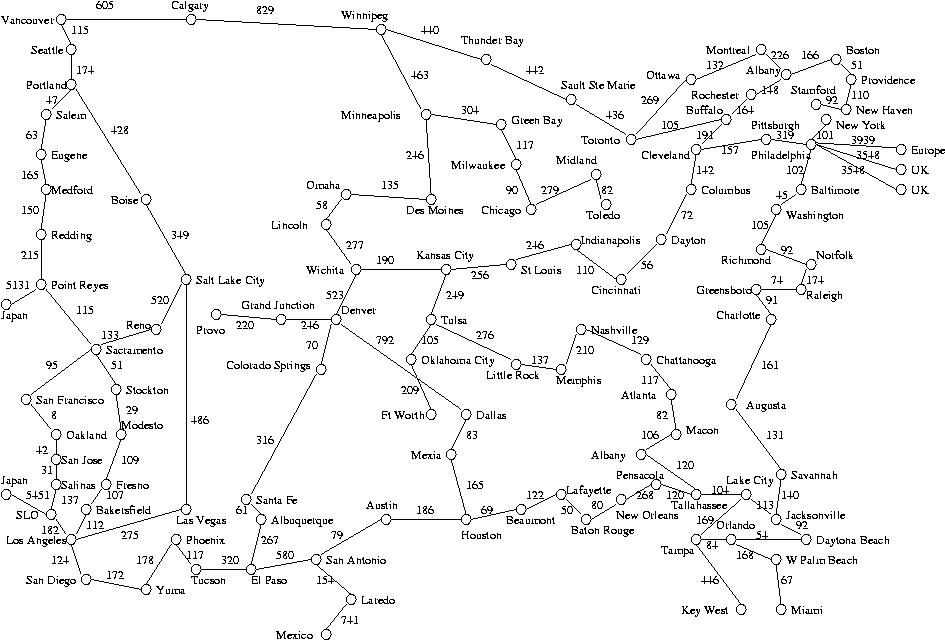
\includegraphics[scale=0.45]{map.jpg}
	\end{center}
	\end{figure} 
	
The road system is implemented as Prolog procedures in usroads.pl. \\
A node is said to be expanded when it is taken off a data structure and its successors generated. In this code, the structure is a priority queue implemented as a sorted list. (There are more efficient ways to implement such queues.) \\
The straight-line distance between cities is computed using decimal degrees of latitude and longitude by heuristic.pl. \\
Using straight-line distance as the heuristic, and starting from the astar.pl implementation, modify the code into a working Prolog implementation of A*, then perform some experiments. \\
The following modifications to the code will be necessary before you start: 
	\begin{enumerate}
  		\item The map indicates distances in miles, while the heuristic code uses kilometers as the units. Change the heuristic code to use miles.
  		\item The heuristic uses 45 degrees North latitude for all node pairs, which doesn't work well in North America. Change the heuristic code to use the average latitude of the two cities instead of 45 degrees.
  		\item Name this new heuristic source file heuristic2.pl. For ease of use, you can keep the procedure name heuristic/3.
	\end{enumerate}
	\textbf{The subproblems: }\\
	\begin{enumerate}
  		\item (10 pts.) Now experiment with executing the combination of astar.pl, usroads.pl, and heuristic2.pl to find various paths, until you understand the meaning of the output. Are there any pairs of cities (A,B) for which the algorithm finds a different path from B to A than from A to B? Are there any pairs of cities (A,B) for which the algorithm expands a different total number of nodes from B to A than from A to B? \\
  		
  		\textbf{Answer:} There are no such pairs of cities (A,B) for which the algorithm finds a different path from B to A than from A to B. The reason is that the heurisic of computing straight line distance in the heuristic2.pl is admissible. 
  		\item (10 pts.) Compare the working of astar.pl with the two heuristics (heuristic1.pl) and (heuristic2.pl) for the same map usroads.pl. Are there differences between the performance of the two heuristics (either the length of the paths or the number of nodes expanded before reaching the final solution)?\\
  		
  		\textbf{Answer:} I found a difference when apply these two heuristics to find path from orlando to lakeCity. heuristic1: $\left[orlando, daytonaBeach, jacksonville, lakeCity \right]$ (cost 259). heuristic2: $\left[orlando, tampa, lakeCity \right]$ (cost 253). The reason is that heuristic1 uses km instead of mile, which overestimates the straightline distance between cities. As a result, heuristc1 is not admissible, thus not able to find optimal path every time.
  		
  		\item (10 pts.) Change the astar.pl code and/or the heuristic2.pl code so as to implement branch-and-bound search, as discussed in the web notes.
  		\item (10 pts.) Do enough exploration to find at least one path that is longer using branch-and-bound than that found using A*, or to satisfy yourself that there are no such paths. Find at least one path that is found by expanding more nodes than the comparable path using A*, or satisfy yourself that there are no such paths. If there is such a path, list the nodes in the path and the total distance.\\
  		
  		\textbf{Answer:} There are no such paths found by branch-and-bound that is longer using branch-and-bound than that found using A*, since both of these two searches find optimal paths. From orlando to lakeCity, branch-and-bound expands more nodes than A*. The nodes expanded by branch-and-bound is \\ $\left[orlando, daytonaBeach, tampa, jacksonville, westPalmBeach,miami \right]$, while the nodes expanded by A* is $\left[orlando, daytonaBeach, tampa, jacksonville \right]$. The path found by branch-and-bound and A* is $\left[orlando, tampa, lakeCity \right]$ (cost 253).
  		
  		
  		\item (10 pts.) Change the astar.pl code and/or the heuristic2.pl code so as to implement greedy search, as discussed in the web notes.
  		\item (10 pts.) Do enough exploration to find at least one path that is longer using greedy search than that found using A*, or to satisfy yourself that there are no such paths. Find at least one path that is found by expanding more nodes than the comparable path using A*, or satisfy yourself that there are no such paths. If there is such a path, list the nodes in the path and the total distance.\\
  		
  		\textbf{Answer:} From orlando to lakeCity, greedy found a longer path than A*. The path found by greedy is $\left[orlando, daytonaBeach, jacksonville, lakeCity \right]$ (cost 259), while the optimal path found by A* is $\left[orlando, tampa, lakeCity \right]$ (cost 253).
  		
  		\item (10 pts.)Change the astar.pl code and/or the heuristic2.pl code so as to implement dynamic programming search, as discussed in the web notes.
  		\item (10 pts.)Do enough exploration to find at least one path that is longer using dynamic programming than that found using A*, or to satisfy yourself that there are no such paths. Find at least one path that is found by expanding more nodes than the comparable path using A*, or satisfy yourself that there are no such paths. If there is such a path, list the nodes in the path and the total distance.
	\end{enumerate}
	
Submit the following:
	\begin{enumerate}
  		\item Submit your modified code for the heuristic. 
		\item Submit your modified code for branch-and-bound, greedy, and dynamic programming As part of your answer, compare the solution paths and explain what happened, especially any weird behavior you might detect. 
	\end{enumerate}
	
	
	\item (35 pts.) Consider the game-tree in the figure below. The leaf node contain the values generated by some unknown static evaluation function. The root node (level 0) represents the current state of the game and agent must pick the next best state to move to.
	%\usepackage{graphics} is needed for \includegraphics
\begin{figure}[h]
\begin{center}
  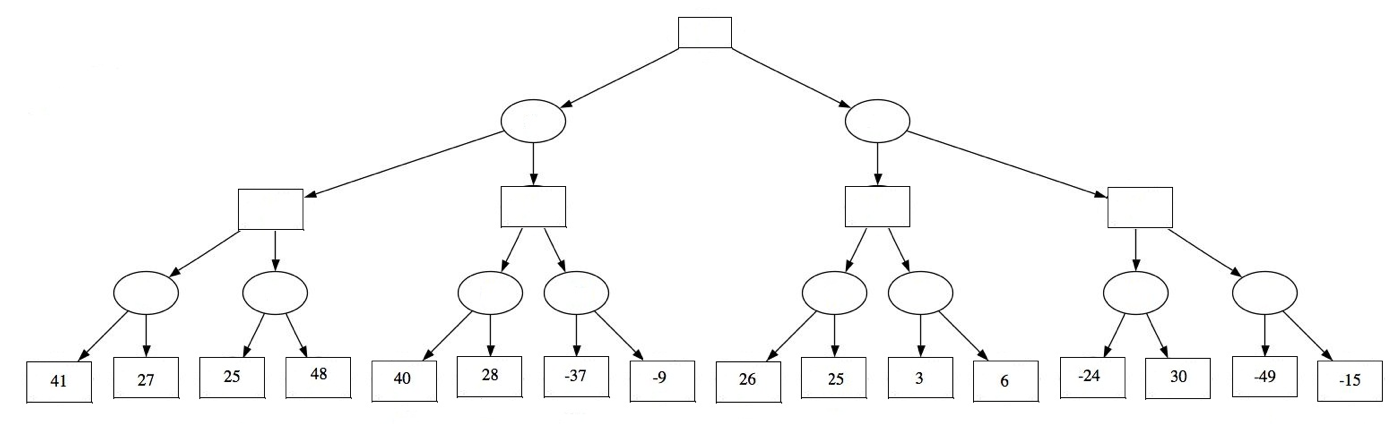
\includegraphics[scale=0.3]{tree.png}
\end{center}
\end{figure}

Now, answer the following questions: \\
	\begin{enumerate}
  		\item (8 pts.) Explore the game-tree just as the agent would using Min-Max algorithm discussed in class. At each level i, indicate the value of the nodes. Indicate the next best state picked by the agent.
  		
\begin{figure}[h]
\begin{center}
  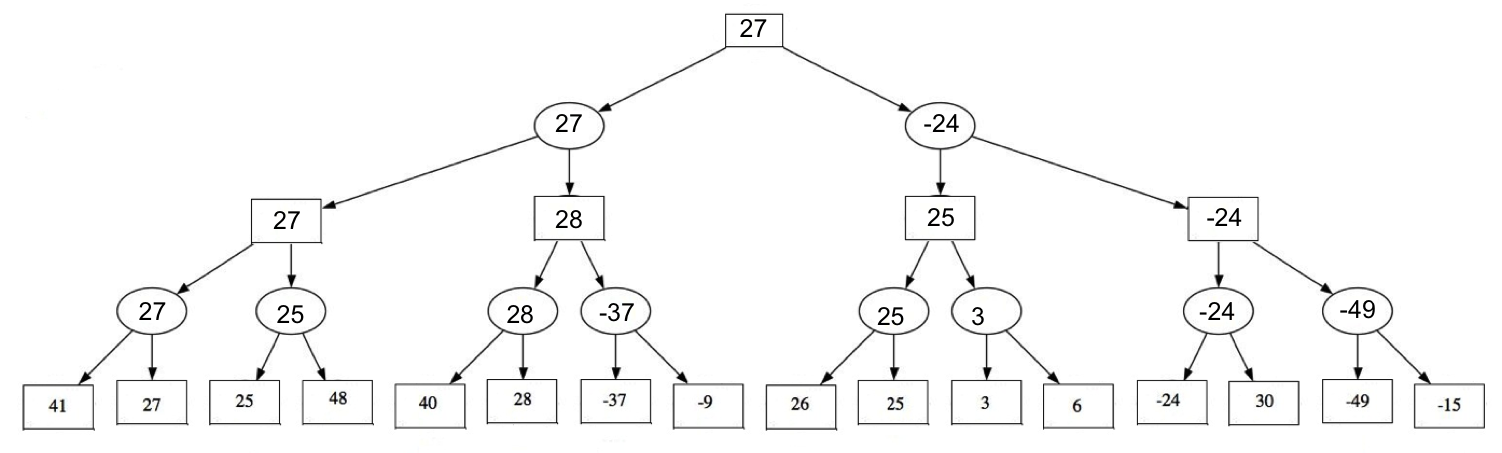
\includegraphics[scale=0.5]{minmax.png}
\end{center}
\end{figure}
  		\item (12 pts.) Explore the game-tree just as the agent would using Alpha-beta pruning discussed in class. At each level i, indicate the value of the nodes and indicate the correct set of nodes that will be pruned. You do not have to label alpha and beta. Indicate the next best state picked by the agent.
\begin{figure}[h]
\begin{center}
  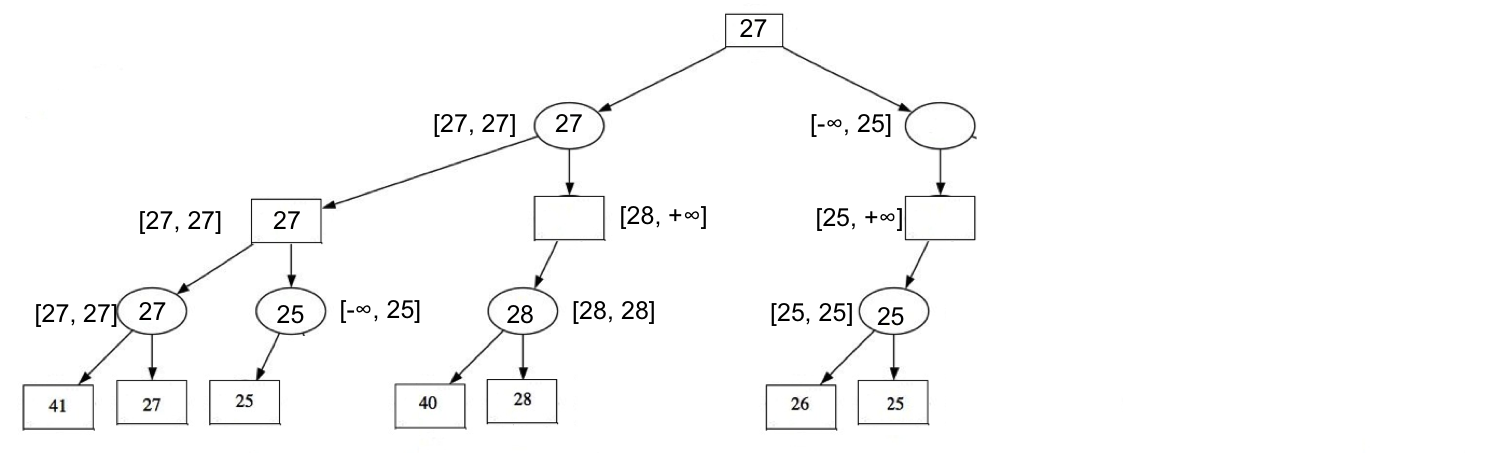
\includegraphics[scale=0.5]{alphabeta.png}
\end{center}
\end{figure} 		
  		\item (5 pts.) What is the worst case for alpha-beta pruning? In the worst case, is the performance of alpha-beta pruning the same as min-max?\\
  		
  		\textbf{Answer:} The worst case for alpha-beta pruning is to expand compute the values of all the nodes. In the worst case, its performance is the same as min-max.
  		
  		\item (10 pts.) Assuming that the values in the leaf nodes, the depth and branching factor remain the same, rearrange the leaves so that the new configuration represents the worst case behavior for alpha-beta pruning. Show the resulting graph and repeat 2b.\\
  		
 \begin{figure}[h]
\begin{center}
  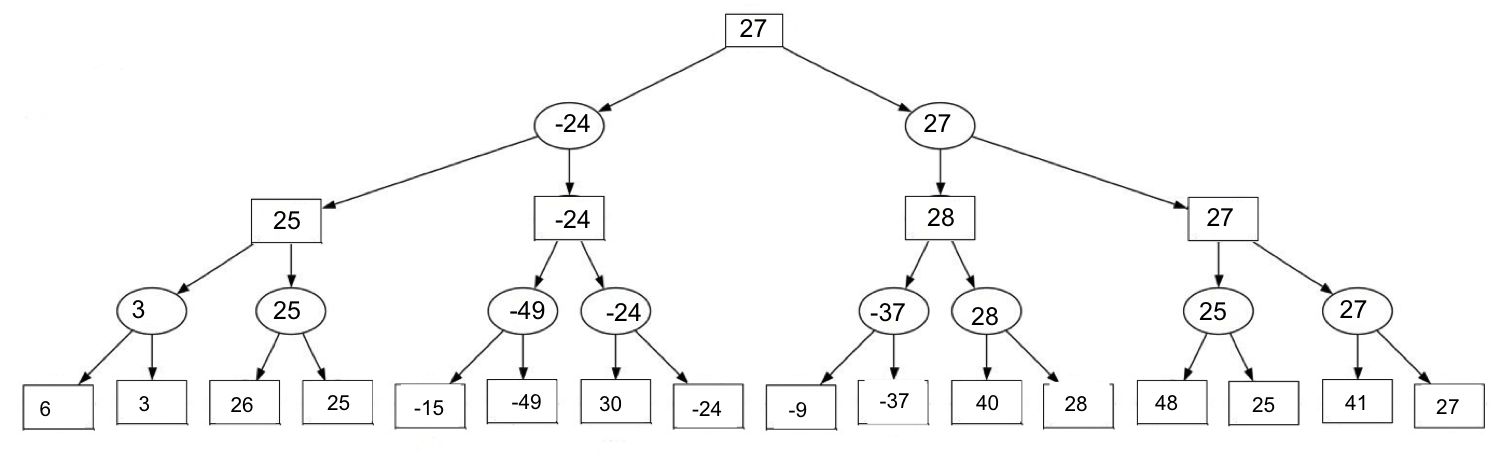
\includegraphics[scale=0.5]{worst.png}
\end{center}
\end{figure} 
	\end{enumerate}

	\item (20 pts.) Ex. 10.4, p. 397 in the textbook.  
\end{enumerate}
\end{document}
